\documentclass{article}

\usepackage{arxiv}

\usepackage[T1]{fontenc}
\usepackage{hyperref}
\usepackage{url}
\usepackage{booktabs}
\usepackage{amsfonts}
\usepackage{amsmath}
\usepackage{amssymb}
\usepackage{nicefrac}
\usepackage{microtype}
\usepackage{cleveref}
\usepackage{graphicx}
\usepackage{natbib}
\usepackage{doi}
\usepackage{xcolor}
\usepackage{tikz}
\usetikzlibrary{arrows.meta,positioning,calc,fit,backgrounds,decorations.pathreplacing}
\usepackage{multirow}
\usepackage{array}
\usepackage{longtable}
\usepackage{float}

\newcommand{\moth}{Moth}
\newcommand{\pp}{\,pp}
\newcommand{\ie}{i.e.,}
\newcommand{\eg}{e.g.,}

\title{Moth: A 19.7\,MB Italian--English Code-Switching Speech Recognizer\\Built on a Pretrained Whisper-Tiny Encoder}

\author{Tancredi Bosi \\
  Semantique \\
  \texttt{tancredi.bosi@gmail.com}}

\date{November 2026}

\renewcommand{\headeright}{A Preprint}
\renewcommand{\undertitle}{A Preprint}
\renewcommand{\shorttitle}{Moth: a 19.7\,MB Italian--English code-switching ASR}

\hypersetup{hidelinks,
  pdftitle={Moth: A 19.7 MB Italian-English Code-Switching Speech Recognizer Built on a Pretrained Whisper-Tiny Encoder},
  pdfauthor={Tancredi Bosi},
  pdfkeywords={speech recognition, code-switching, Italian, English, CTC, Whisper, quantization, edge inference},
}

\begin{document}
\maketitle

\begin{abstract}
Speech recognizers for Italian technical speech must handle English words embedded mid-sentence,
but compact open models often force a single language token per clip and degrade at switches.
We present \moth, a record-then-transcribe Italian--English code-switching ASR system that fits a
hard 20\,MB artifact budget. \moth{} initializes a Whisper-tiny encoder, adds two transformer
blocks and a linear CTC head over a shared 1{,}024-piece Italian+English SentencePiece vocabulary,
and drops the autoregressive decoder and the language token. The released 0.8.1 system has
11.58\,M acoustic parameters and occupies 19.71\,MB: an 11.91\,MB int8 ONNX graph, a 5.38\,MB
trigram language model and a 2.33\,MB Silero VAD. It is trained on 437.7\,h of open
human-transcribed speech, 110\,h of spliced Italian--English exposure and 50.2\,min of recorded mixed speech
oversampled $50\times$, on one
16\,GB laptop with no external compute. On a 600-utterance scripted mixed test set it reaches
24.08\% WER and 55.23\% English-term accuracy; on filtered FLEURS-IT it reaches 20.16\% WER; the
browser path decodes at a median $42\times$ real time in headless Chromium on a desktop. We report the 41-experiment
development record, including rejected quantization-aware training, intermediate CTC, contextual
bias, larger language models and conservative fine-tunes. Decode-side calibration and
language-model data weighting produced the largest measured gains on the mixed test and the rare-term readout, respectively. We also quantify costs hidden
by a single headline number: INT8 adds 0.16\,pp WER on dev and the browser path 0.72\,pp on the
mixed test set; the three voices span 5.34\,pp WER; four seeds of a rejected recipe span 0.46\,pp. All code-switching quality evidence is scripted read speech from three known voices; the public
FLEURS results are read speech from other speakers. The paper makes no claim of spontaneous
code-switching or unseen-speaker generalization on the mixed task.
\end{abstract}

\keywords{speech recognition \and code-switching \and Italian \and CTC \and Whisper \and
quantization \and on-device inference}

\section{Introduction}

Italian technical speech is routinely bilingual: ``ho spostato il \emph{meeting} a domani'',
``mandami il \emph{feedback} sul \emph{deploy}'', ``facciamo un \emph{quick sync} dopo la
\emph{call}''. The English material is not a foreign-language sentence; it is a short, often
domain-specific insertion inside an Italian utterance. A recognizer for this setting must
transcribe both languages with one output stream, must not decide a single language for the whole
clip, and must keep short technical terms intact.

Large multilingual systems handle such input well when they are allowed to be large. The design
constraint here is the opposite: the complete set of required model assets must fit in 20\,MB,
the model must run on a CPU and in a browser tab, and the work must be reproducible on a single
16\,GB laptop with no paid compute. Under that constraint, the standard Whisper recipe is a poor
fit. Its decoder is autoregressive, its checkpoint is 39\,M parameters for the tiny variant, and
its language token is chosen once per 30\,s window---exactly the granularity at which
code-switching happens.

This paper describes \moth{}, a system built around a different decomposition. A pretrained
Whisper-tiny encoder supplies acoustic representations learned from a large, weakly supervised
corpus. Two additional transformer blocks and a linear CTC head map those representations to a
single shared Italian+English SentencePiece vocabulary. There is no decoder and no language
token: every frame emits either a subword or a blank. A small trigram language model is used only
during beam-search decoding, and a voice-activity detector gates silence. The resulting artifact
has 11.58\,M acoustic parameters and occupies 19.71\,MB in its shipped form.

The scientific interest is not the architecture, which is deliberately conventional. It is the
measured development record under a hard byte budget, and the gap between what looks like progress
on a development set and what survives on the deployed artifact. We report 41 experiments,
including twelve rejected interventions. Several plausible improvements---more English data, a
larger vocabulary, intermediate CTC, quantization-aware training, contextual bias, a larger
language model, a conservative knowledge-distilled fine-tune---did not produce a deployable gain.
The largest single improvement on the mixed test came from recalibrating the decoder; the
largest rare-term improvement came from rebuilding the language model from a frozen training-side
corpus with different pruning and term weighting. We quantify both, and we quantify what they
cost.

\paragraph{What the paper reports.}
\begin{itemize}
  \item A complete, open-weight Italian--English code-switching system at 19.71\,MB: 11.58\,M
        acoustic parameters, an 11.91\,MB int8 ONNX graph, a 5.38\,MB trigram LM and a 2.33\,MB
        VAD. It runs record-then-transcribe on CPU and in the browser via ONNX Runtime Web.
  \item Main results on a scripted mixed test set (24.08\% WER, 55.23\% ETA on 600 utterances),
        a never-acoustically-trained voice (24.96\% / 51.27\% on 200 utterances), filtered
        FLEURS-IT (20.16\%), and a comparison against Whisper-tiny, Whistle and Parakeet at
        their measured artifact sizes.
  \item A measured account of decode-side gains, rare-term gains, noise robustness,
        quantization cost and browser cost, each with paired confidence intervals and the
        conditions under which the number was produced.
  \item A negative-results section that separates recipe properties from seed artifacts: the
        rare-term shortfall of the conservative fine-tune reproduces across eight runs, while
        its silence hallucination does not.
  \item An explicit validity boundary. Every code-switching quality number comes from scripted
        read speech and three known voices; the public FLEURS numbers are read speech from other
        speakers. There is no spontaneous code-switching test and no unseen speaker in the mixed
        test.
\end{itemize}

\paragraph{What the paper does not claim.}
It does not claim a new architecture, state-of-the-art accuracy, or general code-switching
competence. It does not claim that the reported comparisons are matched in pretraining data,
compute or decoding budget. It does not treat a confidence interval that includes zero as proof
of equivalence. The system is a small, working artifact and the paper is a case study of how it
was measured.

\section{Related Work}

\paragraph{Code-switching ASR.}
Code-switching has been studied with language-specific acoustic models, language identification,
unified multilingual vocabularies and end-to-end models; \citet{sitaram2019survey} survey the
area. The SEAME \citep{lyu2010seame} and ASCEND \citep{lovenia2022ascend} speech corpora made
Chinese--English switching measurable, and LinCE \citep{aguilar2020lince} centralized text
benchmarks across several language pairs, but Italian--English technical speech remains
comparatively under-resourced. End-to-end Mandarin--English work has examined shared subword
units and language-aware training \citep{zeng2019endtoend}. A recurring finding is
that a single language token or a monolingual decoder forces an unnatural decision at the
utterance level, while a shared subword vocabulary with a frame-synchronous objective avoids
that decision. \moth{} follows the second route: one vocabulary, one CTC output stream, no
language token.

\paragraph{Small and on-device ASR.}
Whisper \citep{radford2023whisper} established robust multilingual ASR from weak supervision, and
its tiny variant is a common starting point for edge systems. Distillation reduces it further \citep{gandhi2023distilwhisper}; Moonshine \citep{jeffries2024moonshine} targets live
transcription with a compact encoder--decoder; on-device engines such as Whistle
\citep{cactus2024whistle} and transducer models in NeMo \citep{nemo2024} provide strong
engineering baselines. Earlier end-to-end systems established recurrent and attention-based
recognition \citep{amodei2016deepspeech2,chan2016las,chiu2018sota}; self-supervised pretraining
\citep{hsu2021hubert} and large multilingual training \citep{zhang2023usm,pratap2023mms} now
supply representations that small systems reuse, and open toolkits such as SpeechBrain
\citep{ravanelli2021speechbrain} make these baselines reproducible. Compression and quantization
\citep{han2016deepcompression,jacob2018quantization,krishnamoorthi2018quantizing} are what make a
sub-20\,MB package practical. Most of these systems are optimized for English or for
broad multilingual coverage; the Italian--English mixed-term case is usually a secondary
condition. \moth{} is intentionally narrower.

\paragraph{CTC and decoding.}
CTC \citep{graves2006ctc} removes the need for frame-level alignment and supports a
non-autoregressive, frame-synchronous encoder. Prefix beam search with an external language model
\citep{graves2012sequence,hannun2014deepspeech} remains an effective decoder for small CTC
models, and intermediate CTC losses \citep{lee2021interctc} are a standard regularizer. CTC was
also extended to end-to-end recurrent models \citep{graves2014towards}, and n-gram language models
remain practical at this scale \citep{kneser1995improved,heafield2011kenlm,sundermeyer2012lstm}.
Our architecture is a plain CTC model; the interesting result is how much of the final quality is
decided by decoder calibration and LM data rather than by the acoustic network.

\paragraph{Evaluation validity.}
Code-switching evaluation is sensitive to the test population: read scripted sentences,
spontaneous conversation and elicited term lists measure different things. LinCE
\citep{aguilar2020lince} makes this explicit by separating tasks and languages. We therefore
report the test population, the reuse history and the per-voice range, and we do not describe the
mixed test set as an untouched natural benchmark.

\section{System}

\subsection{Task and text normalization}

The input is 16\,kHz mono audio, at most 30\,s per request. The output is lowercase text without
punctuation or case restoration. This is a record-then-transcribe system: it is not streaming, it
does not produce word timestamps, and it does not perform diarization.

All training text, LM text and scoring pass through one normalizer. It applies NFKC and
lowercase, folds apostrophes and joins whitespace after them, spells digit sequences with
\texttt{num2words} using the language hint, separates hyphens, dashes and slashes, keeps Latin
letters, Italian accented vowels and apostrophes, folds other Latin diacritics, drops other
symbols and collapses whitespace. Mixed or unknown language falls back to Italian rules. Using
one rule for training and scoring avoids a class of silent mismatch between the acoustic targets
and the reported WER. It also means that punctuation and capitalization are outside the task,
not merely unmeasured.

\subsection{Acoustic model}

\begin{figure}[t]
\centering
\begin{tikzpicture}[
  font=\footnotesize,
  box/.style={draw=black!55, rounded corners=1.2pt, line width=0.45pt,
              minimum height=8.6mm, minimum width=17mm, align=center, inner sep=1.2mm},
  data/.style={box, fill=black!4},
  pre/.style={box, fill=teal!10},
  new/.style={box, fill=orange!12},
  dec/.style={box, fill=blue!6},
  ar/.style={-{Latex[length=1.4mm,width=1.2mm]}, line width=0.5pt, draw=black!70}
]
\node[data] (mel) {log-mel\\$80\times T$, 10\,ms};
\node[data, right=4mm of mel] (stem) {conv stem\\$80\!\to\!384$, $/2$};
\node[pre, right=4mm of stem, minimum width=24mm] (enc) {Whisper-tiny\\block $\times 4$};
\node[new, right=4mm of enc, minimum width=21mm] (extra) {extra block\\$\times 2$};
\node[new, right=4mm of extra] (lin) {linear\\$384\!\to\!1025$};
\node[dec, right=4mm of lin] (ctc) {CTC\\blank $+$ BPE};
\draw[ar] (mel) -- (stem);
\draw[ar] (stem) -- (enc);
\draw[ar] (enc) -- (extra);
\draw[ar] (extra) -- (lin);
\draw[ar] (lin) -- (ctc);
\node[above=1.2mm of stem.north east, anchor=south east, font=\scriptsize, color=black!65]
  {50\,Hz};
\draw[decorate, decoration={brace, amplitude=3pt}, line width=0.4pt]
  ([yshift=-2.5mm]stem.south west) -- ([yshift=-2.5mm]enc.south east)
  node[midway, below=3.2pt, font=\scriptsize, align=center]
  {Whisper encoder, 7.63\,M\\pretrained (MIT)};
\draw[decorate, decoration={brace, amplitude=3pt}, line width=0.4pt]
  ([yshift=-2.5mm]extra.south west) -- ([yshift=-2.5mm]lin.south east)
  node[midway, below=3.2pt, font=\scriptsize, align=center]
  {new head, 3.94\,M\\trained from scratch};
\node[below=11.5mm of enc.south, font=\scriptsize, color=black!70]
  {total acoustic network: 11{,}575{,}169 parameters};
\end{tikzpicture}
\caption{The \moth{} acoustic graph. A log-mel front end feeds a stride-two convolutional stem
and the four pretrained Whisper-tiny encoder blocks. Two additional pre-LayerNorm transformer
blocks and a linear projection produce 1{,}025 CTC classes (blank plus 1{,}024 BPE pieces).
There is no autoregressive decoder and no language token. The graph runs at 50 frames per second;
the 30\,s limit corresponds to 1{,}500 encoder frames. At inference a separate 2.33\,MB Silero VAD
gates silence and optionally segments multi-utterance audio, and a 5.38\,MB trigram LM is used
only inside beam search.}
\label{fig:architecture}
\end{figure}

Figure~\ref{fig:architecture} shows the model. The front end is the Whisper log-mel
representation: 80 bins, 25\,ms window, 10\,ms hop, per-clip dynamic-range normalization. A
two-layer convolutional stem (kernel 3, stride 1 then stride 2, GELU) maps 80 bins to width 384
and halves the frame rate to 50\,Hz. Four pre-LayerNorm transformer blocks follow, each with six
64-dimensional attention heads, a 1{,}536-wide GELU feed-forward network and a final
LayerNorm. Attention is bidirectional and masked by real-frame key padding; it is not causal or
streaming. Positions are fixed sinusoids generated as a non-persistent buffer, not learned
parameters.

The released configuration adds two full transformer blocks after the encoder's final
LayerNorm, then a linear projection to 1{,}025 classes and a float32 log-softmax at inference.
This detail matters: early project notes describe ``a linear CTC head on the Whisper encoder'',
which would be 8.03\,M parameters. The shipped model is 11.58\,M, because the two extra blocks
are part of the trained and exported network. \Cref{tab:params} gives the exact accounting.

\begin{table}[t]
\centering
\small
\caption{Parameter accounting of the released acoustic network. Counts include weights and
biases, exclude buffers, optimizer state, the language model and the separate VAD network.}
\label{tab:params}
\begin{tabular}{@{}lr@{}}
\toprule
Component & Parameters \\
\midrule
Convolutional stem and four pretrained encoder blocks (with final LayerNorm) & 7{,}632{,}384 \\
Two post-encoder transformer blocks ($2\times1{,}774{,}080$) & 3{,}548{,}160 \\
CTC linear projection ($384\times1025+1025$) & 394{,}625 \\
\midrule
\textbf{Total acoustic network} & \textbf{11{,}575{,}169} \\
\bottomrule
\end{tabular}
\end{table}

The blank label is index 0; BPE piece $i$ maps to CTC index $i+1$, including the unknown piece.
The model therefore has no explicit word boundary, no language tag and no punctuation class. The
inductive bias is that mixed Italian--English text is one sequence over one vocabulary.

\subsection{Tokenizer}

The vocabulary is a 1{,}024-piece SentencePiece BPE model \citep{kudo2018sentencepiece} trained on
normalized MLS-IT and LibriSpeech-EN training transcripts, the mixed training pool and a curated
list of 580 English technical terms. Italian is oversampled to 70\% of transcript words (not audio
hours), and the curated terms are weighted to about 5\% of corpus lines. The resulting model
tokenizes at 1.945 tokens per word and 4.70 tokens per second; 48.8\% of the curated English terms
fit in at most three pieces. These are historical build statistics: the serialized tokenizer is
not committed to the repository, and the builder does not promise byte-identical SentencePiece
output across runs. The vocabulary used by the release is pinned through the exported
\texttt{vocab.json}, not through the original SentencePiece model.

\subsection{CTC decoding}

The default decoder is a CTC prefix beam search \citep{graves2012sequence} with beam width 12 and
the top 10 non-blank labels per frame. A trigram BPE language model is combined in shallow fusion,
\begin{equation}
  \log p(\mathbf{y}\mid\mathbf{x}) \;\approx\;
  \log p_{\mathrm{CTC}}(\mathbf{y}\mid\mathbf{x})
  + \alpha \log p_{\mathrm{LM}}(\mathbf{y})
  + \beta\,|\mathbf{y}| ,
\end{equation}
with LM weight $\alpha=0.55$ and per-token bonus $\beta=2.7$. The bonus is not cosmetic. Without
it, an LM trained on text shorter than the acoustic hypothesis penalizes each emitted token, and
the decoder deletes about 12\% of reference words to avoid that penalty. The recalibration that
introduced the bonus moved mass from deletions to insertions and lowered WER by 6--9 points on
every set without changing a single weight (Section~\ref{sec:decoder}).

A greedy CTC decoder is available as a fast path. It uses no LM and no bonus; it is the mode in
which the acoustic model alone is measured. Greedy and beam results are therefore not
interchangeable and are labeled separately throughout.

The LM is a BPE trigram with stupid backoff 0.4, stored as a sparse CSR binary of int16-quantized
log-probabilities. The shipped 0.8.1 LM (arm A3 in E-031) was built from a frozen training-side corpus, keeps all
bigrams while requiring count at least two for trigrams, and repeats term-containing sentences three times.
Section~\ref{sec:rare} isolates what that change did and what it cost.

\subsection{Runtime, VAD and packaging}

At inference a Silero VAD \citep{silero2021vad} runs first. The no-speech gate uses the fraction
of VAD windows above a 0.1 speech-probability threshold; the fraction must exceed 0.10. If at
least two speech runs are found, the runtime transcribes each span separately; a single run is
left intact. Spans shorter than 560 samples or longer than 30\,s are rejected rather than
silently cropped. Segmentation is not diarization.

The acoustic graph is exported to ONNX opset 17 and dynamically quantized to int8. The Python
runtime loads ONNX Runtime sessions, the binary LM and the mel filters once; the browser runtime
loads the same files through ONNX Runtime Web with WASM SIMD. The browser path implements its own
log-mel front end and beam decoder. Audio is processed in the tab and is not uploaded by the demo.

The released package contains seven files. The 20\,MB ceiling is on the sum of these required
assets, not on the browser's JavaScript, the Python environment, or a download-compressed
archive. The shipped 0.8.1 package is 19{,}706{,}289 bytes, leaving 293{,}711 bytes of headroom.
A 25\,MB tier exists in the release validator but was not used.

\section{Data}
\label{sec:data}

\subsection{Open corpora}

Training uses three open human-transcribed sources, summarized with the evaluation sets in
\Cref{tab:data}. Common Voice IT 27 \citep{ardila2020commonvoice} contributes 167.79 manifest
hours (113{,}118 clips), MLS Italian \citep{pratap2020mls} 169.89\,h (40{,}953 clips), and
LibriSpeech train-clean-100 English \citep{panayotov2015librispeech} 100.00\,h (28{,}370 clips).
The natural mixture is 437.68 unique hours, 77/23 Italian/English by audio duration. It is not the
design's shorthand 70/30: reaching 70/30 would either discard more than 100\,h of Italian or
repeat English.

The manifest builder applies deterministic duration sampling (1--30\,s), duration and character
filters, a digit-transcript filter, and a speaking-rate filter. Evaluation manifests and their
normalized-text hashes are built before training, so the overlap check is not retrofitted. The
filtering is why the reported FLEURS populations (697 Italian, 525 English) are smaller than the
upstream test splits.

\begin{table}[t]
\centering
\small
\setlength{\tabcolsep}{3.4pt}
\caption{Data used by the released system. ``Unique'' counts distinct audio; ``exposure'' counts
epoch-weighted repetitions. Spliced material reuses natural clips by construction; gold data are
50.2 unique minutes repeated $50\times$. Total training exposure is 589.55\,h, of which 41.87\,h is
repeated gold. Test sets are never trained on, but T and S3 have informed development repeatedly
(Section~\ref{sec:validity}).}
\label{tab:data}
\begin{tabular}{@{}l>{\raggedright\arraybackslash}p{2.45cm}rrl@{}}
\toprule
Source & License & Unique & Clips & Role \\
\midrule
Common Voice IT 27 & CC0 & 167.79\,h & 113{,}118 & train \\
MLS Italian & CC-BY 4.0 & 169.89\,h & 40{,}953 & train \\
LibriSpeech EN & CC-BY 4.0 & 100.00\,h & 28{,}370 & train \\
Spliced IT+EN & derived & 110.00\,h & --- & train \\
R-S1 + R-S2 gold & recorded, consent & 50.2\,min & 1{,}263 & train ($50\times$) \\
MUSAN + room tone & CC-BY 4.0 / own & 217 clips & 217 & noise aug. \\
\midrule
MLS-IT + LS-EN dev & CC-BY 4.0 & 10.48\,h & 3{,}939 & selection \\
T-600 (S1--S3) & recorded, consent & 23.2\,min & 600 & test (reused) \\
T-S3 & recorded, consent & 7.7\,min & 200 & test (reused) \\
FLEURS-IT test & CC-BY 4.0 & 2.74\,h & 697 & test \\
FLEURS-EN test & CC-BY 4.0 & 1.39\,h & 525 & test \\
CV-IT test & CC0 & 25.81\,h & 14{,}643 & test \\
Silence/noise/music & mixed & 76.2\,min & 457 & non-speech \\
\bottomrule
\end{tabular}
\end{table}

\subsection{Recorded mixed speech}

The only source of genuinely mixed Italian--English audio is a small recorded corpus made for this
project. A generator produced a pool of 3{,}137 sentences in eight categories (control Italian,
control English, single-word insertions, phrases, brands, acronyms, Italianized verbs and
switch-point sentences). A scripted test set T contains 800 sentences, 200 per speaker; 600 were
recorded by S1, S2 and S3 (23.2 minutes total) and the fourth block remains unrecorded. A
separate training script R was recorded by S1 (641 takes) and S2 (622 valid takes), 50.2 unique
minutes in total. An anchor set A has each recorded speaker read 60 T sentences; it is a
script/channel control, not an independent test.

All recordings are 48\,kHz mono, converted to 16\,kHz for training and evaluation. Every take is
bound to a manifest row with text, speaker, category, duration and file hash. The scripts were
reviewed by hand: 1{,}464 lines were read, 24 lines in the unrecorded S4 block were corrected, and
13 recorded R lines with article errors were left untouched because the audio contains the error
and rewriting the text would desynchronize audio and transcript. No recorded row was modified.
There are no category violations, no duplicates and no near-duplicates above trigram Jaccard 0.8
within the scripts.

\subsection{Splicing and noise augmentation}

Two augmentation strategies expand the effective training signal without new recordings.
Utterance-level splicing concatenates an Italian clip and an English clip into one training
example, producing 110\,h of exposure; this teaches the model to switch inside a sequence without
inventing new speech. Splicing reuses the same source sentences, so it is a training-signal
choice, not new data.

Noise augmentation replaces about half of the Common Voice Italian material (83.6\,h) with noisy
versions. The clean/noisy split is derived from a hash of the clip ID, and each noisy clip has a
fixed SNR drawn once in the 10--30\,dB range. Noise comes from a pool of 217 clips: MUSAN noise and
music \citep{snyder2015musan} plus a room-tone recording. Because the SNR is fixed per clip, the
augmentation is deterministic across epochs and does not silently change the difficulty of the
training set between runs. The pool is used in training; the separate held-out room in
Section~\ref{sec:noise} is not.

\subsection{Development and test sets}

Checkpoint selection uses a 3{,}939-clip dev set: 1{,}248 MLS-IT utterances and 2{,}691
LibriSpeech-EN utterances, 10.48\,h in total. The selection metric is the unweighted mean of the
two corpus WERs, not a pooled WER. This choice is deliberate---it prevents the larger English
partition from dominating---but it also means that a dev improvement need not correspond to a
mixed-set improvement. The released model's dev number is slightly worse than its predecessor's
(Section~\ref{sec:lineage}); the product readout, not the dev number, decided adoption.

The product readouts use T-600 (600 scripted mixed utterances, 3{,}488 reference words and 1{,}043
annotated English positions), its S3 subset (200 utterances, 1{,}174 words, 355 English
positions), filtered FLEURS-IT and FLEURS-EN test sets, the full 14{,}643-clip Common Voice IT
test set where historical numbers exist, and a 457-clip non-speech set. T is the only mixed test
set; it is scripted read speech, not spontaneous conversation.

\subsection{Leakage controls and term provenance}
\label{sec:leakage}

The project treats leakage as a property to be audited rather than asserted. Test and dev
manifests were hashed before training. T, R and the sentence pool are disjoint beyond exact
script reuse; the anchor A repeats 60 T sentences by design. A source-level audit hashed 2{,}209
recorded wav files: no hash appears in two sets, every manifest path resolves, and the
train/dev/test ID sets inside Common Voice, MLS and LibriSpeech are disjoint.

A text near-duplicate audit over 247{,}510 documents found 8{,}205 pairs above trigram Jaccard
0.8 after correcting the MinHash implementation. All are explained: spliced training data reusing
LibriSpeech and MLS sentences by construction, Common Voice prompt reuse across speakers, or the
project's own script/manifest pairs. Zero pairs involve T or FLEURS. A raw-audio pass over
287{,}429 loose files (12.8\,GB) found no cross-source byte collisions; the only repeated hashes
are 120 byte-identical silence clips (one signal repeated, relevant when interpreting a silence
probe) and one room-tone recording stored under two names. The held-out room tone used in
Section~\ref{sec:noise} is absent from the training noise pool.

Term provenance required a correction that matters for how the rare-term result is read. T
contains 655 English terms. Against the acoustic source text including LibriSpeech train-clean-100
and the term addenda, they split into 475 natural, 145 gold and 35 terms that were absent from the
0.7.0 training text. The historical rare-term readout is defined on a fixed set of 47
utterances and 81 annotated span tokens so that earlier experiments remain comparable. It is a
fixed metric, not a claim that the shipped 0.8.1 has never seen the vocabulary: all 35 terms were
introduced by the E-015/E-028 addenda, so 0.8.1 has seen them. The earlier ``44 never-seen
terms'' label was too wide because it omitted LibriSpeech; nine of those terms are in
LibriSpeech train-clean-100.

\section{Training}
\label{sec:training}

Experiments are referred to by their retained repository IDs (E-000--E-041); Appendix~\ref{app:experiments}
indexes all of them.

\subsection{Hardware, budget and cost}

All training ran on an Apple M5 MacBook Pro with 16\,GB of unified memory, using PyTorch 2.14.1
with MPS and bf16 autocast; CTC loss is computed in fp32. Long runs used AC power and
\texttt{caffeinate -i}. The external monetary cost was 0\,USD. This is not a claim that the work
was free: it consumed author time and a laptop, and the largest runs took most of a working day.
A feasibility probe (E-000) measured 394\,ms per synthetic step with bf16 on MPS, 812 audio
seconds per wall second, which made the project viable before any real data were trained.

\subsection{Recipe}

The shared recipe is AdamW with betas $(0.9,0.98)$, $\epsilon=10^{-8}$ and weight decay 0.01, a
500-step warm-up, cosine decay to 5\% of peak, gradient clipping at 1.0, and batches capped at
192 audio-seconds or 32 clips. Inputs are truncated to 30\,s. Augmentation is SpecAugment
\citep{park2019specaugment} plus tempo stretch, a standard audio-augmentation recipe
\citep{ko2015audio}; the first full fine-tune (E-005) had an epoch
counter bug that repeated the same augmentation view across epochs, which was fixed afterwards.
Checkpoints are written every 10--20 minutes and selected by dev macro WER. Seed 0 is used for the
released lineage.

\subsection{Lineage}
\label{sec:lineage}

\begin{table}[t]
\centering
\small
\setlength{\tabcolsep}{3.4pt}
\caption{Training lineage. Dev macro WER is the checkpoint-selection metric on 3{,}939
MLS-IT/LS-EN clips. ``Release'' marks the first shipped version whose acoustic weights come from
that arm. The E-024 dev minimum conflicts with the release label (see Appendix~\ref{app:repro}).}
\label{tab:lineage}
\begin{tabular}{@{}llrl>{\raggedright\arraybackslash}p{4.15cm}r@{}}
\toprule
Arm & Initialization & Steps & Change & Dev & Release \\
\midrule
E-004 & converted Whisper & 5{,}871 & frozen encoder, linear head & 75.77 & --- \\
E-005 & E-004 & 72{,}592 & full fine-tune, 437.7\,h & 33.77 & --- \\
E-006 & E-005 & 36{,}296 & $+2$ transformer blocks & 31.27 & --- \\
E-014 & E-006 & 22{,}494 & $+110$\,h spliced IT/EN & 30.86 & --- \\
E-017 & E-014 & 26{,}442 & $+$S1+S2 gold, $50\times$ & 30.98 & 0.5.0 \\
E-024 & E-014 & 26{,}442 & $+$noise augmentation & 30.84 & 0.7.0 \\
E-028 & E-024 & 13{,}283 & $+$S2 term addendum; gentler LRs & 31.01 & 0.8.0/0.8.1 \\
\bottomrule
\end{tabular}
\end{table}

\Cref{tab:lineage} and \Cref{fig:training} summarize the acoustic lineage. The frozen-encoder probe
(E-004) established that the pretrained representation was useful but insufficient: a linear head
on frozen features reached 75.77\% dev WER. Full fine-tuning (E-005) dropped dev WER to 33.77\%
and beat Whisper-tiny on Common Voice dev by 10.9 points, but missed the pre-registered FLEURS-IT
bar by 5.3 points. Adding two transformer blocks (E-006) took dev WER to 31.27\%; adding spliced
Italian--English material (E-014) took it to 30.86\%.

The gold-data arms are the product story. E-017 added S1 and S2's recorded mixed speech, oversampled
$50\times$, and improved T-S3---a speaker with no training audio---by an amount comparable to the
trained speakers (6.1 points, against 4.5 and 6.6), which argued against pure speaker adaptation. E-024 reran the recipe from E-014
with the same gold data and noise augmentation, released as 0.7.0. E-028 then added the S2 term
addendum and lowered the learning rates (encoder $10^{-5}$, head $10^{-4}$) for one epoch, 13{,}283 steps; it is the
acoustic model in 0.8.0 and 0.8.1.

\begin{figure}[t]
\centering
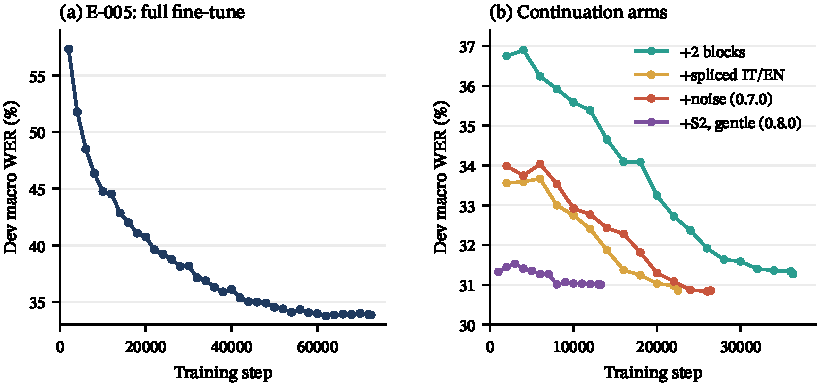
\includegraphics[width=\textwidth]{figures/fig_training.pdf}
\caption{Dev macro WER from the retained training logs. (a) The from-scratch full fine-tune
E-005: the first dev point is 57.3\% at step 2{,}000; the curve reaches 33.77\% at 72{,}592 steps.
(b) Continuation arms. E-028 starts at the 0.7.0 dev level (30.81\%), rises to 31.53\% under the
initial optimization shock, and returns to 31.01\%---slightly worse than its parent. It was
adopted on product readouts, not on dev.}
\label{fig:training}
\end{figure}

\subsection{Selection, gates and the dev/product gap}

Adoption decisions were made against written plans; the later arms used pre-registered gates. The E-028 arm,
for example, had six gates: rare aligned ETA at least 30\%, T-600 ETA at least 53.7\%, T-600 WER
at most 25.7\%, at least 431 of 817 natural-term occurrences, FLEURS-IT/EN not worse by more than
0.5 points with a CI excluding zero, and a checkpoint selected by dev rather than the step-20
baseline. The fp32 candidate passed all six; the first int8 export missed the rare gate by one
aligned occurrence, and the published 0.8.0 decoder arm by two (23/81 against the required 25/81). That exception was documented at publication rather than redefined after
the fact.

The dev metric and the product metric are not the same quantity. E-028's dev WER is 0.20 points
worse than 0.7.0, while its T-600 and T-S3 results are better. The project kept the dev set as a
selection tool and treated the product readout as the decision, but this is a real weakness: a
model that improves the target behavior can look worse on a proxy that weights pure Italian and
pure English read speech. Section~\ref{sec:validity} returns to this point.

\section{Evaluation Protocol}
\label{sec:protocol}

\paragraph{Word error rate.}
WER is computed after normalization, by minimum edit distance over words, from summed
substitutions, deletions and insertions divided by reference words. Corpus WER is not the mean of
per-utterance WERs. The T-600 reference has 3{,}488 words; a one-word change moves corpus WER by
about 0.03\,pp, so small point differences should not be read as precise.

\paragraph{English-term accuracy (ETA).}
ETA is the fraction of annotated English-origin reference positions reproduced exactly after
alignment. It is a strict exact-match metric, not semantic equivalence. On T-600 there are 1{,}043
annotated positions. The rare-term readout uses 81 annotated span tokens in the 47 rare-bearing
utterances (47 target tokens plus 34 co-occurring annotated tokens), and a separate presence
count over the 47 utterances. Presence and aligned ETA answer different questions and are
reported separately. The 81 tokens are not 81 independent terms.

\paragraph{Confidence intervals.}
Unless stated otherwise, intervals are 95\% percentile intervals from 1{,}000 paired
utterance-level bootstrap resamples with seed 0, following standard bootstrap practice for ASR and
MT evaluation \citep{efron1993bootstrap,bisani2004bootstrap,koehn2004statistical}. The resampling unit is
the utterance, not the speaker, seed or recording session. A CI that includes zero is called a
\emph{tie}; this means no detected difference at this sample size, not equivalence and not
non-inferiority. Intervals for per-speaker results are within-speaker intervals and do not
estimate between-speaker variance. The multi-seed result in Section~\ref{sec:speakers} is a
descriptive range over four replicates, not a variance estimate.

\paragraph{Baselines.}
Whisper-tiny \citep{radford2023whisper} is evaluated in fp32 on CPU, padded to 30\,s, with no
hotwords. We report forced-Italian beam-5 on T (the better language setting for mixed speech) and
automatic-language beam-5 on FLEURS (the best measured variant). Whistle \citep{cactus2024whistle}
is evaluated with its native engine, forced Italian, no hotwords; the engine's exact kernel
precision and beam are not recorded in the baseline metadata. Parakeet TDT 0.6B v3 is evaluated
as an int8 transducer through NeMo/sherpa-onnx with greedy search and four threads
\citep{nemo2024}. These are engine comparisons, not matched-compute or matched-pretraining
experiments.

\paragraph{Artifact sizes.}
Sizes are declared artifact bytes, not parameter counts and not full runtime footprints. For
\moth{} the number is the sum of the seven required release files. For the baselines it is the
serialized model artifact recorded in the baseline metadata: 148.7\,MB of fp32 parameter storage for Whisper-tiny,
16.9\,MB for Whistle's compressed engine file and 670.5\,MB for Parakeet's serialized export. These quantities exclude
different things (tokenizer, VAD, runtime libraries, compression), so \Cref{fig:size} is a
size--accuracy sketch, not a controlled efficiency benchmark.

\section{Results}
\label{sec:results}

\subsection{Main results}

\begin{table}[t]
\centering
\small
\setlength{\tabcolsep}{4pt}
\caption{Main comparison. \moth{} numbers are the shipped 0.8.1 int8 graph with the A3 LM and
decoder 12/10/0.55/2.7. Whisper uses forced-Italian beam 5 on T and automatic-language beam 5 on
FLEURS (its best FLEURS variant); Whistle is forced Italian; Parakeet is int8 greedy. T-S3
baselines were not measured for Parakeet. Artifact sizes are declared bytes and are not
like-for-like (Section~\ref{sec:protocol}).}
\label{tab:main}
\begin{tabular}{@{}lrrrrrr@{}}
\toprule
System & T-600 WER & T-600 ETA & T-S3 WER & T-S3 ETA & FLEURS-IT & Size \\
\midrule
Whisper-tiny & 50.72 & 36.05 & 46.51 & 38.03 & 27.42 & 148.7\,MB \\
Whistle & 29.42 & 49.28 & 28.36 & 52.11 & 11.85 & 16.9\,MB \\
Parakeet TDT 0.6B & 10.98 & 83.60 & --- & --- & 3.65 & 670.5\,MB \\
\textbf{\moth{} 0.8.1} & 24.08 & 55.23 & 24.96 & 51.27 & 20.16 & 19.7\,MB \\
\bottomrule
\end{tabular}
\end{table}

\begin{figure}[t]
\centering
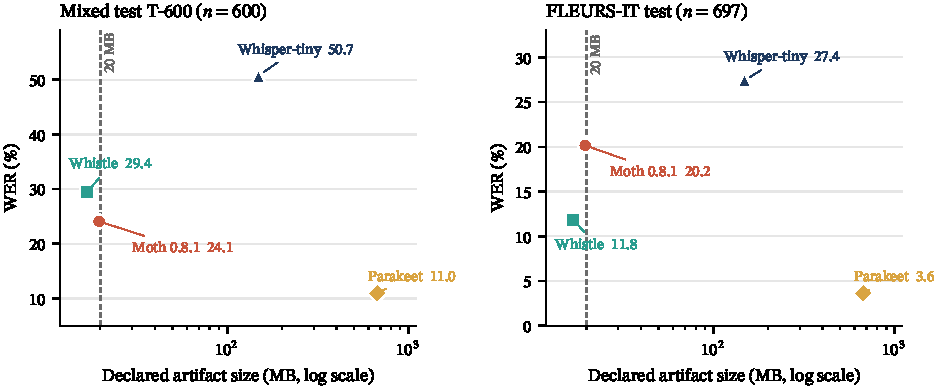
\includegraphics[width=\textwidth]{figures/fig_size_wer.pdf}
\caption{WER against declared artifact size, on a logarithmic axis. Left: the scripted mixed test
T-600. Right: filtered FLEURS-IT. The dashed line marks the 20\,MB ceiling. At 19.7\,MB \moth{} has the best mixed-set WER in
this comparison: Whisper and Parakeet are 7.5$\times$ and 34$\times$ larger, and Whistle is
2.8\,MB smaller but 5.3\,pp worse on the mixed set. The FLEURS panel shows the
cost of specialization: \moth{} beats Whisper-tiny on Italian read speech but is far behind
Whistle and Parakeet, and its pure-English FLEURS WER is 49.81\% (not shown).}
\label{fig:size}
\end{figure}

\Cref{tab:main} and \Cref{fig:size} give the headline comparison. On the mixed scripted set,
\moth{} reaches 24.08\% WER and 55.23\% ETA. It beats Whisper-tiny by 26.6\,pp WER and 19.2\,pp
ETA, and Whistle by 5.3\,pp WER and 6.0\,pp ETA. Parakeet remains far better (10.98\% WER,
83.60\% ETA) at roughly 34 times the artifact size. On FLEURS-IT, \moth{} beats Whisper-tiny
(20.16 vs 27.42) but is worse than Whistle (11.85) and Parakeet (3.65). On FLEURS-EN it is poor
(49.81\%) because the acoustic mixture is Italian-dominant and the English training material is
audiobook speech, not the read FLEURS domain.

Two cautions apply to every row. First, the baselines may have seen FLEURS or its source material
during pretraining; we cannot audit upstream contamination. Second, the T-600 aggregate is not a
speaker-independent estimate. S1 and S2 contributed acoustic training audio (400 of 600 clips);
S3 contributed none but shares S1's microphone family and has been inspected repeatedly. The
per-voice breakdown in Section~\ref{sec:speakers} is part of the result, not an appendix.

\subsection{Decoder calibration}
\label{sec:decoder}

\begin{figure}[t]
\centering
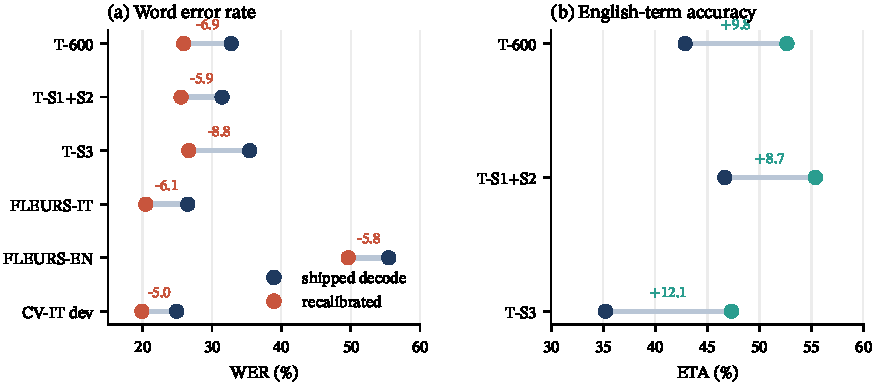
\includegraphics[width=\textwidth]{figures/fig_decoder.pdf}
\caption{Decoder recalibration on unchanged acoustic weights (E-022). The shipped decode used beam
5, top-8, LM weight 0.2 and no token bonus; the recalibrated decode uses beam 12, top-10, LM
weight 0.5 and a per-token bonus of 2.4. (a) WER drops on all six sets; every paired CI excludes
zero. (b) ETA rises on all three T subsets. The mechanism is visible in the error mix:
deletions fall from 12.2\% to 8.3\% of reference words and insertions rise from 0.8\% to 1.3\%.
The artifact and the int8 graph are byte-identical between the two decodes.}
\label{fig:decoder}
\end{figure}

The largest single measured improvement on the mixed test came from decoding, not training.
\Cref{fig:decoder} shows E-022: on unchanged E-017 weights, a wider beam, a stronger LM weight and
a per-token bonus reduced T-600 WER from 32.77\% to 25.92\% and raised T-S3 from 35.43\% to
26.66\%. FLEURS-IT fell from 26.52\% to 20.46\%, crossing the Whisper-tiny bar that had blocked
the project. All six sets improved with paired CIs excluding zero. The ETA gain was 9.8 points on
T-600 and 12.1 on T-S3.

The mechanism was a length bias. The LM had been trained on text shorter than the acoustic
hypotheses, so its per-token log-probability penalized every extra token. The decoder responded by
deleting words. Adding a constant bonus per emitted token compensates the bias without changing
the acoustic model or the LM. Deletions fell by about a third and insertions rose slightly; total
errors fell. This is a calibration fix, not a modeling insight, and it cost zero bytes.

A second recalibration (E-030) moved the shipped decoder to LM weight 0.55 and bonus 2.7,
selected on a 1{,}277-clip dev set, and recovered most of the int8 gap of the E-028 acoustic arm.
The shipped 0.8.1 decoder is 12/10/0.55/2.7. The fact that two rounds of decoder tuning produced
more than any single acoustic arm is a statement about this model at this scale, not a general
claim that decoding is more important than acoustics.

\subsection{Rare English terms}
\label{sec:rare}

\begin{figure}[t]
\centering
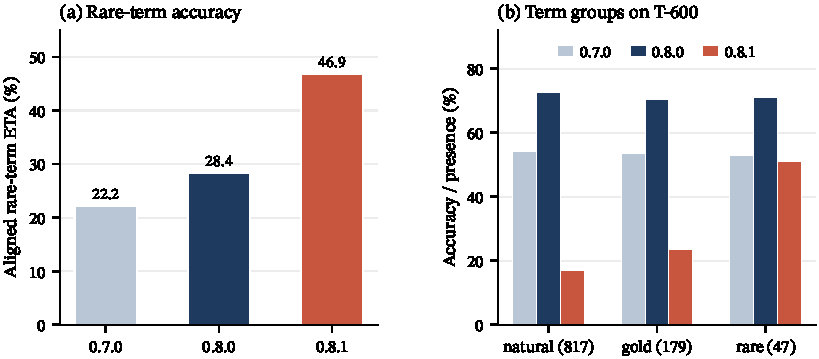
\includegraphics[width=\textwidth]{figures/fig_rare.pdf}
\caption{(a) Aligned rare-term ETA over the fixed 47-utterance / 81-token readout. (b) Exact-match
accuracy by term group on T-600. Bars are Moth 0.7.0, 0.8.0 and 0.8.1. Natural and gold are occurrence-level exact-match rates;
rare is utterance-level presence. The 0.8.1 LM rebuild raises rare-term presence from 23.4\% to 51.1\% while giving back 9
natural-term occurrences; the gold group is essentially unchanged. The rare group is 47
utterance-level checks, not 47 independent terms.}
\label{fig:rare}
\end{figure}

\begin{table}[t]
\centering
\small
\setlength{\tabcolsep}{4pt}
\caption{Rare-term readout and term groups for the three published releases. Aligned ETA and
presence use the fixed historical definition; provenance was corrected after the 0.8.1 release
(Section~\ref{sec:leakage}). ``16-term'' is a separate regression set.}
\label{tab:rare}
\begin{tabular}{@{}lrrrrrr@{}}
\toprule
Release & Aligned ETA & Presence & Rare WER & Natural & Gold & 16-term \\
\midrule
0.7.0 & 22.2\% (18/81) & 8/47 & 40.2\% & 441/817 & 130/179 & 22/27 \\
0.8.0 & 28.4\% (23/81) & 11/47 & 35.9\% & 436/817 & 126/179 & 19/27 \\
0.8.1 & \textbf{46.9\% (38/81)} & \textbf{24/47} & \textbf{28.2\%} & 432/817 & 127/179 & 19/27 \\
\bottomrule
\end{tabular}
\end{table}

The intended use case includes short English terms that are rare in the training text. The project
therefore tracks a fixed rare-term readout: 47 T utterances that contain at least one of the
terms absent from the 0.7.0 acoustic training text. \Cref{tab:rare} and \Cref{fig:rare} show the
progression across releases.

The 0.8.1 gain is decode-side. The acoustic graph is byte-identical to 0.8.0. The LM was rebuilt
from a frozen training-side corpus with three simultaneous changes: all bigrams were kept,
trigrams still required count at least two, and term-containing sentences were repeated three
times. The binary grew to 5{,}381{,}992 bytes, still inside the package budget. Aligned rare ETA
rose from 28.4\% to 46.9\% (23/81 to 38/81, $+18.5$\,pp, CI $[+9.6,+31.0]$), presence from 11/47
to 24/47, and rare WER from 35.9\% to 28.2\%. T-600 as a whole improved by 0.63\,pp WER and 1.06\,pp
ETA, both with CIs excluding zero; T-S3 and FLEURS were ties.

The cost is visible in the same table: natural-term occurrences fell from 436 to 432 (and from
441 at 0.7.0), and the 16-term regression set stayed at 19/27 after dropping from 22/27 at 0.7.0.
The LM change is therefore not a free win; it trades a small amount of broad vocabulary coverage
for a large gain on the targeted terms. The three build changes are confounded: the experiment
does not isolate corpus refresh, pruning and term weighting. A later attempt to spend the
remaining 293{,}711 bytes on 73{,}427 additional count-1 trigrams (E-035) improved dev macro WER
by 0.06\,pp but produced a tie on every product metric and was rejected.

The rare-term metric also needed a provenance correction. After including LibriSpeech
train-clean-100, 35 terms across 37 T utterances---not 44 across 47---were genuinely absent from
the 0.7.0 text, and all 35 were introduced by the term addenda that 0.8.1 trained on. The
historical 47/81 readout is retained for comparability, but it is no longer evidence that the
shipped model has never seen the vocabulary. This distinction does not change any measured value;
it changes the sentence that the values support.

\subsection{Noise robustness}
\label{sec:noise}



Noise augmentation (E-024) is the intervention with the clearest practical effect.
\Cref{fig:noise} and \Cref{tab:noise} compare 0.6.0 and 0.7.0 on the same 100 S3 clips. On the
shared pool, the gain is significant at 15, 10 and 5\,dB: $-6.28$, $-11.54$ and $-9.68$ points.
At 30 and 20\,dB the differences are ties, and the clean condition is 1.70 points worse (CI
includes zero). On a room recorded after training---and confirmed by the audio audit to be absent
from the training noise pool---the relative gain is larger at every noisy condition
($-3.90$ to $-18.34$ points). The room is also harder in absolute terms: 36.50\% WER at 15\,dB
against 27.33\% on the shared pool. Both facts belong together; quoting only the larger gain
would overstate absolute robustness.

The caveats are substantive. The shared-pool estimate reuses noise clips that were in training,
so it may be optimistic. The held-out room is one 38\,s take; its conditions and utterances are
correlated, and it is not a sample of rooms. SNR is RMS-relative, not active-speech SNR or a
measured acoustic condition. The ETA intervals all include zero. The noise test therefore supports
a claim about this augmentation recipe on this protocol, not a general far-field robustness
claim.

\begin{figure}[t]
\centering
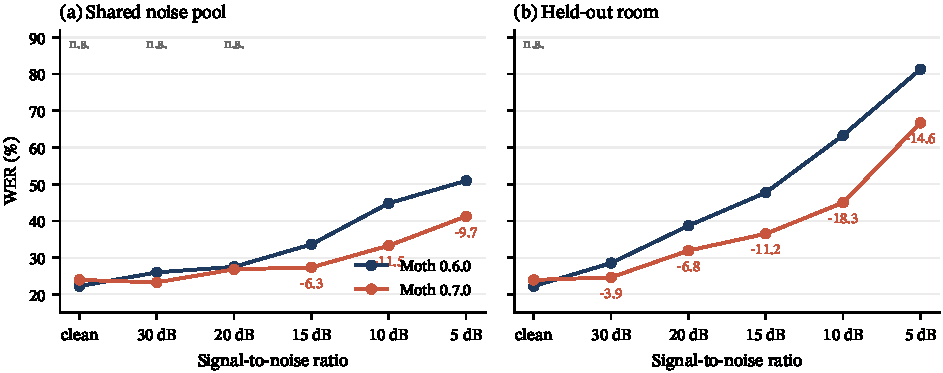
\includegraphics[width=\textwidth]{figures/fig_noise.pdf}
\caption{Noise curves for 0.6.0 (E-017 weights) and 0.7.0 (E-024 weights) on the first 100 S3
clips. (a) Shared noise pool, used in training. (b) Room recorded after training and absent from
the training pool. Annotations show significant WER deltas in percentage points; ``n.s.'' marks
conditions whose paired CI includes zero. The new room is harsher in absolute terms: at 15\,dB it
is 36.50\% WER for 0.7.0, against 27.33\% on the shared pool.}
\label{fig:noise}
\end{figure}

\begin{table}[t]
\centering
\small
\setlength{\tabcolsep}{4pt}
\caption{Noise WER (\%) for the 0.6.0$\to$0.7.0 comparison. Each condition uses the same 100 S3
clips and 589 reference words. The shared-pool estimate is potentially optimistic because all
pool clips were used in training; the held-out room is one 38\,s take, not a room population.}
\label{tab:noise}
\begin{tabular}{@{}lrrr@{\hspace{1.1em}}rrr@{}}
\toprule
& \multicolumn{3}{c}{Shared pool} & \multicolumn{3}{c}{Held-out room} \\
\cmidrule(lr){2-4}\cmidrule(lr){5-7}
SNR & 0.6.0 & 0.7.0 & $\Delta$ & 0.6.0 & 0.7.0 & $\Delta$ \\
\midrule
clean & 22.24 & 23.94 & $+1.70$ & 22.24 & 23.94 & $+1.70$ \\
30\,dB & 25.98 & 23.26 & $-2.72$ & 28.52 & 24.62 & $-3.90$ \\
20\,dB & 27.50 & 26.83 & $-0.68$ & 38.71 & 31.92 & $-6.79$ \\
15\,dB & 33.62 & 27.33 & $-6.28$ & 47.71 & 36.50 & $-11.21$ \\
10\,dB & 44.82 & 33.28 & $-11.54$ & 63.33 & 44.99 & $-18.34$ \\
5\,dB & 50.93 & 41.26 & $-9.68$ & 81.32 & 66.72 & $-14.60$ \\
\bottomrule
\end{tabular}
\end{table}

\subsection{Quantization and deployment}
\label{sec:deploy}

\begin{figure}[t]
\centering
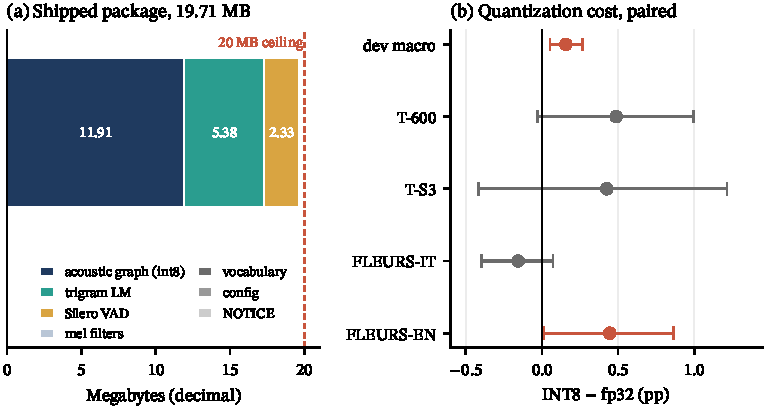
\includegraphics[width=\textwidth]{figures/fig_package.pdf}
\caption{(a) Composition of the shipped 0.8.1 package: 19.71\,MB, with 293{,}711 bytes of headroom
under the 20\,MB ceiling. (b) Paired INT8$-$fp32 WER difference with the same E-028 checkpoint,
A3 LM and decoder. Positive means INT8 is worse. Filled markers are intervals that exclude zero.
The cost is small on dev, larger on T-600 and FLEURS-EN, and slightly negative on FLEURS-IT: it is
not a uniform shift.}
\label{fig:package}
\end{figure}

The shipped graph is dynamically quantized int8. E-037 measured what that costs by decoding the
same checkpoint through the fp32 export and the int8 graph with the same A3 LM and decoder
(\Cref{fig:package}b). On the 3{,}939-clip dev set, macro WER rises from 22.8596\% to 23.0170\%
(+0.1574\,pp, CI $[+0.0539,+0.2664]$). On T-600 the point estimate is +0.4874\,pp (CI
$[-0.0290,+0.9963]$, a tie) with ETA $-0.8629$\,pp; T-S3 is a tie at +0.4259\,pp. FLEURS-EN is
significantly worse (+0.4459\,pp, CI $[+0.0087,+0.8652]$), while FLEURS-IT is slightly better
($-0.1559$\,pp, tie). Rare-term hits are unchanged at 38/81, and the noise word count is slightly
better under int8. The cost is real, small, and non-uniform. The fp32 package would be
54{,}164{,}659 bytes, so int8 is the only deployable format; the measurement documents the price
of the ceiling rather than justifying a change.

The browser path adds a second, different cost. E-041 decoded T-600 through the shipped bundle in
headless Chromium with ONNX Runtime Web: 24.7993\% WER and 54.3624\% ETA, against 24.0826\% and
55.2253\% from the Python runner. The WER difference is +0.7167\,pp with CI $[0.0000,+1.4723]$
(touching zero), ETA $-0.8629$\,pp (tie), and 151 of 600 hypotheses differ. The penalty is not
uniform: S1 +0.26\,pp WER, S2 +0.35\,pp, S3 +1.53\,pp and $-2.82$\,pp ETA. The never-trained voice
pays five to six times the WER cost of the trained voices.

This is a deployment property, not a model-quality claim. The browser uses a different log-mel
implementation and different WASM kernels; the decoder itself is exact on identical logits, and
the runtime acceptance suite passes 4/4 configurations (isolated 1/4 threads and non-isolated).
Median RTFx was 42.3 in the first browser run (range 25.5--53.4) and 44.87 on the post-merge
rerun that pinned the release (range 24.89--59.96), on a desktop with 10 hardware threads; the two
runs produced identical hypotheses. The 0.8.1 acceptance fixture measured medians of 46.69, 46.23,
25.10 and 24.83 across four configurations. These are desktop measurements, not phone, Safari or
end-user latency claims.

\subsection{Speaker and seed variability}
\label{sec:speakers}

\begin{figure}[t]
\centering
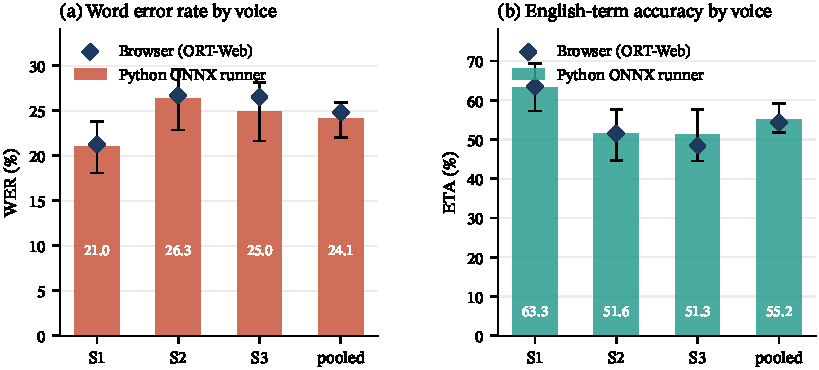
\includegraphics[width=\textwidth]{figures/fig_speakers.pdf}
\caption{Per-voice results for the shipped 0.8.1, with within-speaker 95\% bootstrap intervals.
Bars are the Python ONNX runner; diamonds are the browser path. S1 and S2 contributed acoustic
training audio; S3 did not. The pooled number is an average over these three voices, not a
speaker-independent estimate.}
\label{fig:speakers}
\end{figure}

\begin{figure}[t]
\centering
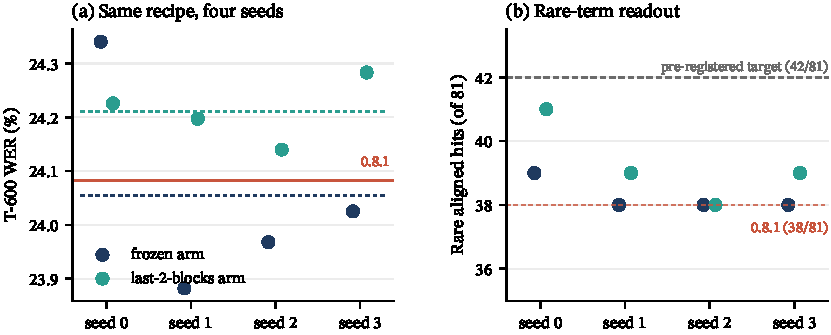
\includegraphics[width=\textwidth]{figures/fig_seeds.pdf}
\caption{(a) T-600 WER of the rejected E-036 conservative fine-tune, four seeds per arm. The
between-seed range of the frozen arm (0.4587\,pp) is larger than the gap between arms
(0.1577\,pp). (b) Rare-term aligned hits for the same runs. No replicate reaches the
pre-registered 42/81 target; the shortfall is a recipe property. The silence hallucination of
E-036 did not reproduce (Section~\ref{sec:negative}).}
\label{fig:seeds}
\end{figure}

\Cref{fig:speakers} shows the per-voice result. Pooled T-600 is 24.08\% WER and 55.23\% ETA, but
S1 is 20.98\% / 63.28\%, S2 is 26.32\% / 51.56\% and S3 is 24.96\% / 51.27\%. The voices span
5.34\,pp WER and 12.02\,pp ETA. The never-trained S3 is not the worst voice; S2 is. With three
voices, between-speaker variance is not estimable and a speaker-cluster interval cannot be formed.
The per-voice intervals overlap, so the ordering is descriptive. The correct sentence is: on the
three available voices the model ranges from 20.98\% to 26.32\% WER and from 51.27\% to 63.28\%
ETA; the pooled 24.08\% / 55.23\% is an average over voices.

Training-seed variability was measured only for the rejected E-036 recipe, not for the released
0.8.1 lineage. Four seeds of each of two conservative arms produced T-600 means of 24.0539\% and
24.2116\%, with within-arm ranges of 0.4587\,pp and 0.1434\,pp (\Cref{fig:seeds}). The gap between
the two arms (0.1577\,pp) is smaller than the frozen arm's seed range, so the arm ordering carried
no information. The same runs show that the rare-term shortfall reproduces (no replicate reaches
42/81) while the silence hallucination does not (four of eight replicates emit nothing on all 120
silence clips). The released model's single seed is therefore a limitation, not an estimated
variance: 0.46\,pp is the scale at which small acoustic differences should be treated as noise in
this recipe family.

\section{Negative Results}
\label{sec:negative}

\begin{table}[t]
\centering
\footnotesize
\setlength{\tabcolsep}{2.6pt}
\caption{Rejected interventions. Each row has a written plan and a retained result; the outcome
column reports the measured value that decided the rejection. These are not equal-budget
controlled comparisons, and several are single-seed probes.}
\label{tab:negative}
\begin{tabular}{@{}p{0.9cm}>{\raggedright\arraybackslash}p{3.0cm}>{\raggedright\arraybackslash}p{4.9cm}l@{}}
\toprule
ID & Intervention & Measured outcome & Decision \\
\midrule
E-012 & $+200$\,h LibriSpeech EN & FLEURS-EN $-5.4$ points, but T $+5.16$ worse and ETA flat & rejected \\
E-013 & BPE 4{,}096 & FLEURS-IT $+1.9$ worse, T flat, ETA unchanged, $+1.2$\,M params & rejected \\
E-015 & first gold-term addendum & rare $8\to11/47$, CI includes zero; FLEURS worse; dev 33.64 & rejected \\
E-019 & Whistle LoRA probe & S3 $+2.30$ WER; FLEURS/CV significantly worse; 28\,MB export & rejected \\
E-023 & full (unpruned) LM & dev $-0.65$ but 12.31\,MB binary, 26.63\,MB package & rejected \\
E-027 & decode-time contextual bias & rare ETA 22.22\%$\to$22.22\%; T-600 +0.10 (tie) & rejected \\
E-029 & quantization-aware training & best probe T-600 25.34 vs 25.14 gate & rejected \\
E-032 & targeted S1 term addendum & rare up, but T-S3, FLEURS and natural terms down; 6 gates failed & rejected \\
E-033 & intermediate CTC (weight 0.3) & dev $+0.0249$\,pp, CI $[-0.0998,+0.1557]$ & rejected \\
E-034 & larger n-gram LM & dev $-0.6$\,pp, but 12.0--12.3\,MB binary; package 26.4\,MB & rejected \\
E-035 & budgeted count-1 trigrams & dev $-0.0645$\,pp; product tie on all primary metrics & rejected \\
E-036 & conservative KD fine-tune & rare 39/81 and 41/81 vs 42 target; T-S3 ETA $-1.41$ & rejected \\
E-040 & four-seed replication & arm gap below seed noise; silence bimodal & no adoption \\
\bottomrule
\end{tabular}
\end{table}

\Cref{tab:negative} lists the rejected interventions. Three clusters are worth reading in detail.

\paragraph{Data and capacity.}
Adding 200\,h of English (E-012) improved English read speech but moved the model away from
Italian and made T-600 5.16 points worse; the English-term accuracy did not move. A larger BPE
vocabulary (E-013) shortened the English terms but did not teach the acoustic model to emit them,
and Italian regressed. The first gold-term addendum (E-015) was too aggressive: rare terms rose
from 8/47 to 11/47 with a CI including zero, natural terms fell from 439 to 423, FLEURS
regressed, and dev jumped from 30.81\% to 33.64\%. These results are consistent with a capacity
and mixture problem that a single lever cannot fix.

\paragraph{Regularization, quantization and distillation.}
Intermediate CTC (E-033) learned its auxiliary objective (loss 66.9 to 0.72 over 394{,}625
parameters) but produced no dev gain: +0.0249\,pp with CI $[-0.0998,+0.1557]$. Quantization-aware
training (E-029) closed the int8--fp32 dev gap in a short probe but failed the product gates on
T-600, rare terms and natural terms. The conservative fine-tune (E-036) is the most instructive
negative. It protected WER---dev and product WER were ties---but did not reach the rare-term
target (39/81 and 41/81 against 42/81), and at seed 0 it emitted the token ``x'' on all 120
silence clips. A four-seed replication (E-040) then showed that the rare shortfall is a property
of the recipe while the silence failure is a seed draw: four of eight replicates were clean. The
lesson is not that the recipe was good; it is that a single-seed negative result would have
supported the wrong generalization in both directions.

\paragraph{Language model and decode-time bias.}
A larger unpruned LM (E-023) was worth about 0.65 points on dev but produced a 26.63\,MB package,
over the ceiling. A 12\,MB LM with more trigram coverage (E-034) was also worth about 0.6 points
on dev and also did not fit. The budgeted variant (E-035) fit at 19{,}999{,}997 bytes and improved
dev by 0.06\,pp, but the product readout was a tie on all primary metrics; it was rejected rather
than shipped because a tie does not justify spending the last 3 bytes of margin. Decode-time
contextual bias with a 24-term glossary (E-027) left the rare terms exactly unchanged and was
rejected. The successful LM change (E-031) was not ``more LM'': it was a different corpus
treatment and term weighting inside the existing budget.

\paragraph{What the pattern does and does not show.}
The negative results are not a controlled comparison of architecture families. E-019 used a
different model, data exposure and update budget; E-029 was a short probe; E-033 changed one
regularization weight; E-036 changed several recipe details at once. The defensible pattern is
narrower: in this project, at this scale and under this byte budget, small dev gains repeatedly
failed to survive the product readout, and decode-side changes produced larger measured gains than
the acoustic interventions that were tried. That is a statement about this development record, not
a universal ranking of techniques.

\section{Validity and Discussion}
\label{sec:validity}

\paragraph{What the evidence supports.}
The evidence supports the following statements. A configured 11.58\,M-parameter CTC model and a
19.71\,MB package were built, trained, exported and run on CPU and in Chromium. On scripted mixed
speech from three known voices, the released model reaches 24.08\% WER and 55.23\% ETA, with a
per-voice range of 20.98--26.32\% WER. It beats the measured Whisper-tiny and Whistle baselines on
the mixed set and beats Whisper-tiny on FLEURS-IT, while remaining far behind Parakeet. Noise
augmentation improved WER at 15, 10 and 5\,dB on a paired protocol, including a room recorded
after training. The int8 graph costs about 0.16\,pp on dev and the browser path about 0.72\,pp on
T-600; both are measured, not assumed. The rare-term LM change raised aligned ETA from 28.4\% to
46.9\% at a cost of nine natural-term occurrences.

\paragraph{Construct validity.}
The core construct is ``Italian speech with English words mixed in''. T is scripted read speech,
not spontaneous conversation. It was generated from a sentence pool, reviewed by hand and recorded
in a quiet room. It contains controlled categories (single words, phrases, brands, acronyms,
Italianized verbs, switches) but not the disfluencies, repairs, overlapped speech or topic drift
of natural code-switching. ETA measures exact reproduction of annotated English-origin positions,
not whether the term was understood. The 47-utterance rare subset is a diagnostic, not a
representative sample of Italian technical vocabulary.

\paragraph{Internal validity.}
T and S3 have informed development repeatedly. T is not an untouched final test, and S3 is not an
unseen speaker: it contributed no acoustic training audio but shares S1's microphone family and
has been inspected across many experiments. The anchor A repeats 60 T sentences, so it cannot
serve as independent dev. Checkpoint and decoder selection used dev and, for later arms, product
readouts; the project pre-registered gates, but the sequence of experiments is adaptive. The
released acoustic model has one training seed. The multi-seed evidence comes from a rejected
recipe, not from the release lineage.

\paragraph{External validity.}
There are three voices, all recorded for this project, and no fourth voice exists in the
repository. The per-voice range is descriptive and cannot be extrapolated to a speaker population.
There is no spontaneous mixed-dev and no new-voice holdout; the owner decided not to record more
data. The browser measurements are desktop Chromium with WASM threads, not mobile browsers,
Safari, live microphone capture or end-user latency. The noise evidence is one held-out room and
synthetic RMS-relative SNR, not a corpus of real noisy environments.

\paragraph{Statistical validity.}
The bootstrap resamples utterances, not speakers, seeds or sessions. The intervals are therefore
within-corpus intervals; they do not license inference to new speakers or new rooms. ``Tie''
means ``the interval includes zero at this sample size'', not equivalence. Multiple comparisons
were not corrected; the paper reports the pre-registered primary readouts and labels exploratory
ones. Several effects are small enough that seed variation of the order of 0.46\,pp could matter.
The 81 rare span tokens are correlated within 47 utterances, and the 47 utterances are not 47
independent terms.

\paragraph{Upstream contamination.}
Whisper-tiny, Whistle and Parakeet were pretrained on large, partly undisclosed corpora. FLEURS
and Common Voice are public and may overlap with pretraining data. We can audit local audio and
text leakage, and we did, but we cannot audit upstream pretraining. The FLEURS comparisons should
be read with that uncertainty.

\paragraph{Practical lessons.}
Four lessons generalize beyond this model. (1) Calibrate the decoder before judging the acoustic
model: a length-biased LM can hide several points of WER, and the fix costs no bytes. (2) Under a
hard byte budget, LM corpus composition and weighting can be a better use of the last few hundred
kilobytes than another acoustic block or a larger vocabulary. (3) A dev metric that is not the
product metric can rank models backwards; report both and decide on the product readout. (4) Small
gains need multiple seeds and per-voice reporting; a single-seed tie or win is weak evidence, and
a single-seed hallucination can be a draw rather than a recipe property.

\paragraph{Ethics, licenses and privacy.}
The code is Apache-2.0; the initial encoder weights are MIT; the data licenses are recorded in the
release NOTICE. Recorded speakers consented to the use of their audio for model development. The
browser demo processes audio locally and does not upload it. The model is intended for dictation
and note-taking, not for surveillance, speaker identification or medical/legal transcription. It
has no diarization and no word timestamps, and it should not be used on speech from people who did
not consent to being recorded.

\section{Conclusion}

\moth{} is a 19.71\,MB Italian--English code-switching recognizer built from a pretrained
Whisper-tiny encoder, two additional transformer blocks and a linear CTC head over a shared
vocabulary. It reaches 24.08\% WER and 55.23\% English-term accuracy on a 600-utterance scripted
mixed test set, 20.16\% WER on filtered FLEURS-IT, and runs at a median $42\times$ real time in
headless Chromium on a desktop. The paper documents the full path to that artifact: 41 experiments, twelve rejected
interventions, two decoder recalibrations, a noise-augmentation recipe, an LM rebuild that closed
the rare-term gap, and a measured account of what int8 and the browser cost.

The result is deliberately bounded. The code-switching evidence is scripted read speech from
three known voices; the public FLEURS numbers are read speech from other speakers. There is no
spontaneous code-switching test, no unseen speaker in the mixed test and no speaker-cluster interval.
The released acoustic model has one seed. Those are not minor caveats to be buried in an appendix;
they define what the headline numbers mean. Within that boundary, the system is a useful small
model, and the development record is a concrete example of how much of the outcome was decided by
measurement discipline---decoder calibration, LM data treatment, pre-registered gates and
negative-result replication---rather than by adding parameters.

\paragraph{Artifacts.}
The released model and demo are available at
\url{https://huggingface.co/semantique-team/moth-stt}. The repository retains the experiment
ledgers, per-utterance hypotheses, comparison JSON, release records and the scripts that generate
every figure in this paper. Checkpoints, raw audio and mel shards are not versioned; the paper and
the retained artifacts distinguish what can be re-scored from what can be retrained.

\section*{Acknowledgements}

We thank the three speakers who recorded the T and R sets and consented to their use for model
development, and the maintainers of Whisper, FLEURS, Common Voice, MLS, LibriSpeech, MUSAN,
Silero VAD and ONNX Runtime. No external funding was used; all training ran on the author's
laptop.

\bibliographystyle{unsrtnat}
\bibliography{references}

\appendix

\section{Release Manifest}
\label{app:release}

\begin{table}[H]
\centering
\small
\setlength{\tabcolsep}{4pt}
\caption{The seven required files of \moth{} 0.8.1. The package sum is 19{,}706{,}289 bytes;
the payload excluding \texttt{config.json} and \texttt{NOTICE} is 19{,}701{,}706 bytes. Full
SHA-256 values are retained in \texttt{runs/E-031/release-0.8.1.json}; the two most important are
shown in the text.}
\label{tab:release}
\begin{tabular}{@{}lrl@{}}
\toprule
File & Bytes & Role \\
\midrule
\texttt{model.int8.onnx} & 11{,}910{,}677 & int8 acoustic graph \\
\texttt{lm\_bpe3.bin} & 5{,}381{,}992 & trigram LM, sparse int16 CSR \\
\texttt{silero\_vad.onnx} & 2{,}327{,}524 & Silero VAD v5 \\
\texttt{mel\_filters.bin} & 64{,}320 & 80$\times$201 float32 filterbank \\
\texttt{vocab.json} & 17{,}193 & exported CTC piece map \\
\texttt{config.json} & 1{,}323 & version, decoder and hashes \\
\texttt{NOTICE} & 3{,}260 & attributions \\
\midrule
\textbf{Total} & \textbf{19{,}706{,}289} & 293{,}711 bytes of headroom \\
\bottomrule
\end{tabular}
\end{table}

The int8 graph SHA-256 is
\texttt{7bbfad7e288640538c5c0147f81738bfd63021727b8760b1f3cbbcc4f939764d}; the A3 LM SHA-256 is
\texttt{3be1177b0ca9f18343efb8d00f0d96365226595c9de32d992720aa4e0b0f16f1}. The model was published
on 12 November 2026 and verified live on Hugging Face; hashes pin content consistency, not
publisher authenticity or an immutable external timestamp.

\section{Experiment Index}
\label{app:experiments}

\begin{longtable}{@{}p{1.05cm}>{\raggedright\arraybackslash}p{5.0cm}>{\raggedright\arraybackslash}p{8.0cm}@{}}
\caption{All executed experiment IDs, with the question or intervention and the outcome. E-018 was
planned but never executed because it required a fourth speaker. ``Closed'' means the option was
rejected or exhausted for this recipe; it does not mean the idea is false in general.}
\label{tab:experiments} \\
\toprule
ID & Question / intervention & Outcome \\
\midrule
\endfirsthead
\toprule
ID & Question / intervention & Outcome \\
\midrule
\endhead
\bottomrule
\endfoot
E-000 & Mac feasibility (MPS, bf16) & 394\,ms/step synthetic; feasible \\
E-001 & Baseline matrix (Whisper, Whistle, Parakeet) & measured; FLEURS-IT bar corrected to 27.42 \\
E-002 & Corpus, manifests, mel cache & 509.8\,h cached; splits hashed before training \\
E-003 & int8 export and browser smoke & 8.32\,MB; 33--74$\times$ RTFx \\
E-004 & Frozen encoder probe & dev 75.77; padded and truncated equivalent \\
E-005 & Full fine-tune, 437.7\,h & dev 33.77; FLEURS-IT gate failed by 5.3 \\
E-006 & $+2$ transformer blocks & dev 31.27; adopted \\
E-007 & CTC beam and hotwords & small WER gain; hotwords neutral \\
E-008 & Trigram LM in shallow fusion & dev 27.05; adopted; FLEURS-IT still behind Whisper \\
E-009 & Real-weight int8 export and browser RTFx & 54--66$\times$ (4 threads); adopted \\
E-010 & Browser beam and LM quality path & tie with Python; adopted \\
E-011 & Silence/noise/music robustness & beam+LM hallucinated on silence; VAD added later \\
E-012 & $+200$\,h LibriSpeech EN & English better, Italian/T worse; rejected \\
E-013 & BPE 4{,}096 & FLEURS-IT worse, ETA flat; rejected \\
E-014 & Spliced IT+EN, 110\,h & dev 30.86; adopted \\
E-015 & First gold-term addendum & rare CI includes zero, FLEURS worse; rejected \\
E-016 & S1 gold fine-tune & dev 30.90; adopted path to E-017 \\
E-017 & S1+S2 gold, S3 held out & T-600 32.77; 0.5.0 \\
E-018 & Gold scaling to S4 & never executed \\
E-019 & Whistle LoRA probe & S3 worse, FLEURS/CV worse; rejected \\
E-020 & End-to-end int8 WER cost & +0.17 T-600 tie; FLEURS-IT +0.32 \\
E-021 & fp32 export gap diagnosis & single-draw tail; seeded gate adopted \\
E-022 & Decoder recalibration & $-6.85$ T-600, $-8.77$ T-S3; 0.6.0 \\
E-023 & LM re-tune with calibrated decoder & optimum unchanged; larger LM over budget \\
E-024 & Noise augmentation, half CV-IT & $-11.54$ at 10\,dB; 0.7.0 \\
E-025 & Held-out room noise test & gain larger; absolute WER worse; no new weights \\
E-026 & Rare-term diagnostic & LM is the lever, not top-k; 41/47 reachable \\
E-027 & Contextual bias pilot & rare unchanged; rejected \\
E-028 & S2 term addendum + gentler fine-tune & rare 30.9\%; six gates in fp32; 0.8.0 \\
E-029 & QAT probe & no publishable candidate; closed \\
E-030 & Decoder recalibration for int8 & 5/6 gates; published 0.8.0 \\
E-031 & Frozen-corpus LM rebuild & rare 46.9\%, T-600 24.08; 0.8.1 \\
E-032 & S1 term addendum & rare up, six gates down; rejected \\
E-033 & Intermediate CTC & dev $+0.0249$\,pp, tie; closed \\
E-034 & Larger n-gram LM & $-0.6$ dev, 26.4\,MB package; rejected \\
E-035 & Budgeted count-1 trigrams & $-0.0645$ dev, product tie; rejected \\
E-036 & Conservative KD fine-tune & rare shortfall; rejected \\
E-037 & Paired fp32/INT8 cost & +0.1574\,pp dev; INT8 remains \\
E-038 & Per-speaker T-600 & 5.34\,pp WER, 12.02\,pp ETA range \\
E-039 & Leakage and provenance audit & no literal leakage; 44$\to$35 term correction \\
E-040 & Four-seed replication of E-036 & rare reproduces, silence does not \\
E-041 & Browser acoustic WER/ETA & +0.7167\,pp tie; S3 pays the most \\
\end{longtable}

\section{Reproduction Notes}
\label{app:repro}

The repository separates what can be re-scored from what can be retrained. Per-utterance
hypotheses, metrics, comparison JSON and release records are retained; checkpoints, raw audio, mel
shards and the serialized tokenizer are not versioned. A clean clone can therefore reproduce the
scoring and every figure in this paper from the retained JSON and logs, but it cannot retrain the
model without the external data, the converted Whisper encoder, the gold recordings and the
checkpoints.

Three provenance issues are recorded rather than smoothed over. First, the 0.7.0 release record
labels the selected checkpoint step as 26{,}442, while the training log's minimum dev WER is at
step 26{,}000; the checkpoint hash is not retained, so the discrepancy cannot be resolved from
this checkout. Second, the 0.8.1 model is a decode-only update: the acoustic graph is byte-identical
to 0.8.0 and only the LM and version string changed. Third, ``never seen'' in the rare-term
literature means never seen by 0.7.0, not by 0.8.1; the corrected count is 35 terms across 37
utterances after including LibriSpeech.

Figure~\ref{fig:training} is generated from \texttt{runs/*/train.log.jsonl}. The remaining
figures are generated by \texttt{paper/figures/make\_figures.py} from the retained JSON in
\texttt{runs/E-024}, \texttt{E-031}, \texttt{E-037}, \texttt{E-038} and \texttt{E-040}, with
values that have no machine-readable file transcribed from the named result reports. The
paper is compiled with the arXiv-style \LaTeX{} template \citep{arxivstyle} and
\texttt{tectonic}.

\end{document}
